% !TEX encoding = UTF-8 Unicode
\graphicspath{{figuras/}}

\chapter{Introdução \label{cap1}}

O Relatório Técnico Final é um documento em que o leitor encontra todas as informações técnicas sobre o trabalho desenvolvido. 
O relatório deve conter os seguintes tópicos:
\begin{itemize}\item {\bf Capa ou página de título: } deve conter o nome da instituição, o título (e subtítulo) do projeto, os autores e supervisores, local e data. O título é considerado o resumo mais sintético do projeto e, portanto, é imprescindível que inclua o assunto ou o tópico e a proposta do mesmo. Verifique ainda se o título é: suficientemente preciso, fácil para ler e entender, e  estruturado para o tema e a audiência. 
\item {\bf Contra-capa: } mesma informação da capa mais as assinaturas dos autores.
\item {\bf Sumário: } Enumeração das principais divisões (capítulo, seções, artigos, etc.) do documento, na mesma ordem em que a matéria nele se sucede; visa a facilitar visão do conjunto da obra e a localização de suas partes, e, para tanto, deve aparecer no início da publicação e indicar, para cada parte, a paginação (Dicionário Aurélio, 1999).
\item {\bf Abstract:} é um resumo sucinto do trabalho que serve como um guia para a leitura do relatório. A leitura do abstract deve indicar se vale ou não a pena ler o relatório. 
O abstract pode ser de dois tipos:

\begin{itemize}
  \item Abstract descritivo que responde a questão: qual é o escopo do relatório?
    \item Abstract informativo que responde a questão: quais são os pontos mais importantes apresentados no relatório.
\end{itemize}

\item {\bf Introdução:} uma introdução bem escrita deve abordar os seguintes itens:
  \begin{itemize}
  	\item o assunto  	\item a proposta ou proposição
	\item Objetivos: 
	Enumere uma lista com bullets. Recomenda-se iniciar os itens com verbos no infinitivo. É imperativo manter o paralelismo de linguagem, i.e. se o primeiro item inicia-se com um verbo no infinitivo, todos os demais itens devem também iniciar com verbos no infinitivo!
  	\item o "background" ou fundamentos do projeto  	\item o escopo  	\item a organização do relatório 	 \item os termos chaves
  \end{itemize}
	  \item {\bf Descrição da metodologia:} descreva os métodos usados para executar o projeto.  \item {\bf Apresentação dos resultados}  \item {\bf Conclusões:} conclua baseado nos resultados apresentados, comentando todos os objetivos propostos.  \item {\bf Sugestões e recomendações}  \item {\bf Apêndices:} nomenclatura utilizada (vide exemplo) e material de suporte ou complementação do corpo do relatório, e.g. diagramas de circuitos, códigos de programas desenvolvidos, etc.  \item {\bf Referências bibliográficas}.
\end{itemize}

Um livro clássico mas difícil de ler e entender é \cite{Astrom:1970}, mas também clássico e muito bom é \cite{Astrom:1997}.

Note que figuras são referenciadas com o rótulo {\it figura} seguindo de uma referência numérica sem parênteses, e.g. Mostra-se na figura \ref{fig_cap1_MBPC_blk_diag} um diagrama em blocos de uma arquitetura de controle de processos genérica.

A referência a uma equação é feita usando numeração entre parênteses, e.g. a equação \bref{eq_piuBella} é uma das mais belas equações matemáticas.

\begin{equation}
 \frac{dy}{dt} = A y.   
 \label{eq_piuBella}
\end{equation}


\begin{figure}[!htbp]
\centering
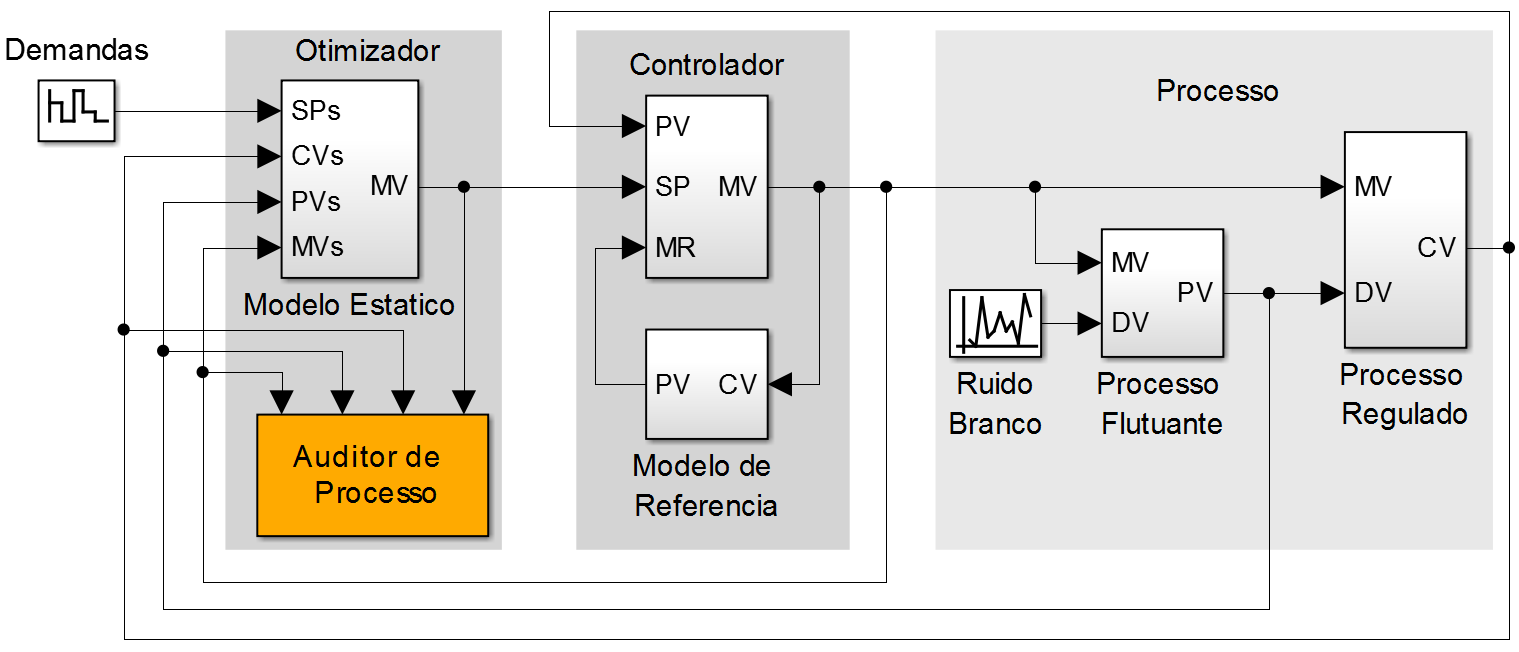
\includegraphics[width=15cm]{cap1_MBPC_blk_diag} 
\caption{Arquitetura simplificada de um sistema de controle baseado em modelo com a função de Auditor de Processo.}
\label{fig_cap1_MBPC_blk_diag}
\end{figure}


\section{Contribuições}

As principais contribuições apresentadas neste trabalho são destacadas abaixo para cada capítulo.

\begin{itemize}

  \item \textbf{Capítulo \ref{cap1}}. Neste capítulo contribuiu-se a partir de uma revisão da literatura...
  
  \item \textbf{Capítulo \ref{cap2}}. Descreve-se...
  
  \item \textbf{Capítulo \ref{cap3}}. Apresenta-se...
  
  \item \textbf{Capítulo \ref{cap4}}. No capítulo 4 é apresentada ...
  
  \item \textbf{Capítulo \ref{cap5}}. No capítulo 5 é apresentada ...
  
\end{itemize}


Conclusões e sugestões de trabalho futuro são apresentadas no Capítulo \ref{cap6}.